\documentclass[11pt,a4paper,titlepage]{article}
\usepackage[a4paper,top=2.5cm,bottom=2.5cm,left=2.5cm,right=2.5cm]{geometry}
%\usepackage{scicite}
\usepackage{times}
\usepackage{hyperref}
\usepackage{setspace}
\usepackage{amsmath}
\usepackage{listings}
\usepackage{graphicx}
\usepackage{enumitem}
\usepackage{tabularx,ragged2e}
\usepackage{geometry}
\usepackage{booktabs}
\usepackage{subcaption}
\usepackage{mwe}
\usepackage{todonotes}

\newcolumntype{L}{>{\RaggedRight\arraybackslash}X}

\makeatletter
\renewcommand*\env@matrix[1][*\c@MaxMatrixCols c]{%
  \hskip -\arraycolsep
  \let\@ifnextchar\new@ifnextchar
  \array{#1}}
\makeatother


\newenvironment{sciabstract}{%
\begin{quote} \bf}
{\end{quote}}



\title{FYS4150 Project 5 - Simulations of monetary transactions using Monte Carlo methods} 
\author
{Mikkel Killingmoe Christensen\\
\\
\normalsize{\today}
}


\date{}

%%%%%%%%%%%%%%%%%%%%%%%%%%%%%%%%%%%%%%%%%%%%%%%%%%
%%%%%%%%%%%%%%%%% END OF PREAMBLE %%%%%%%%%%%%%%%%
%%%%%%%%%%%%%%%%%%%%%%%%%%%%%%%%%%%%%%%%%%%%%%%%%%


\begin{document} 


\maketitle 





\begin{center}
{\large \textbf{Abstract}}
\end{center}
\begin{sciabstract}
Wealth inequality is a huge problem in the world today, and good models  for the economics behind this could be useful to improve the situation. In this project, a model mimicing monetary transactions between agents in a simple economy was made and implemented in C++ using Monte Carlo methods. The model was based on the work by Patriarca et. al \cite{Patriarca} and Goswami and Sen \cite{Goswami}. The model was gradually expanded upon to include savings and biases based on wealth similarity and transaction history. This allowed us to analyze the impact of these biases on the distribution of wealth. It was found that wealth was unevenly distributed when using the model without biases. By adding a parameter for savings, the wealth inequality was reduced. Introducing biases based on wealth similarity, on the other hand, increased the inequality.  Adding a bias based on transaction history agian reduced the inequality, especially when the bias for wealth similarity was high. Furthermore, the tails of some of the distributions were found to fit Pareto distributions \cite{Pareto}. The results were similar to the mentioned articles, but some discrepancies were found, possibly due to the lack of some essential experimental data in the articles making them difficult to reproduce.  
\end{sciabstract}

\tableofcontents
\clearpage


%%%%%%%%%%%%%%%%%%%%%%%%%%%%%%%%%%%%%%
%%%%%%%%%%%Introduction%%%%%%%%%%%%%%%
%%%%%%%%%%%%%%%%%%%%%%%%%%%%%%%%%%%%%%
\section{Introduction}
In this project thesis, concepts from statistical mechanics are used to build a model for monetary transactions between financial agents. This will allow us to numerically study the relation between micro-dynamic relationships among finanicial agents and the resulting macroeconomic money distribution. The theory is based on work by Patriarca et al. \cite{Patriarca}, Goswami and Sen \cite{Goswami} and Pareto \cite{Pareto}, and forms the basis for the model in this project. The agent model will be built up consecutively, adding more and more features. It will start by only including simple transactions without any biases, before it eventually includes saving and transaction preferences among the agents. A description of how the model is implemented using Monte Carlo methods in C++ will also be given. Lastly, the results will be presented and discussed, and compared to the studies the project is based on. 


%%%%%%%%%%%%%%%%%%%%%%%%%%%%%%%%%%%%%%
%%%%%%%%%%%Theory%%%%%%%%%%%%%%%%%%%%%
%%%%%%%%%%%%%%%%%%%%%%%%%%%%%%%%%%%%%%
\section{Theory}
\subsection{Simple model for monetary transactions}
The framework of Patriarca et al. \cite{Patriarca} will be used to simulate the monetary transactions between the agents in the model. I assume that there are $N$ agents exchanging money in pairs of $(i,j)$, and that all agents starts with an initial amount of money $m_0 > 0$. For every cycle, a pair of agents are picked randomly, and a transaction will take place between them. An important property of the transaction is the fact that money is conserved. This is shown in the following equation:
\begin{equation}
\label{eq:money_cons}
m_{i}^{'} + m_{j}^{'} = m_{i}+m_{j},
\end{equation}
where $m_{i}^{'}$ and $m_{j}^{'}$ is the updated wealth of agent $i$ and $j$, and $m_{i}$ and $m_{j}$ is the money they had previous to the transaction. 

The exchange happens through a random reassignment number $\epsilon$, so that:
\begin{equation}
m_{i}^{'} = \epsilon(m_{i}+m_{j})
\end{equation}
\begin{equation}
m_{j}^{'} = (1-\epsilon)(m_{i}+m_{j}).
\end{equation}
The agents will never have debt, that is $m\geq0$. Furthermore, the system reaches an equilibrium caused by the conservation law in equation  \ref{eq:money_cons} given by a Gibbs distribution:
\begin{equation}
\label{eq:Gibbs_dist}
w_{m} = \beta e^{-\beta m}, \ \, \beta = \frac{1}{\langle M\rangle},
\end{equation}
where $\langle M\rangle$ is the average money given by $\langle M\rangle = \sum_i m_i/N = m_0$. After an equilibrium is reached, the majority of the agents is left with lower wealth than they initially had, and the number of rich agents exponentially decrease. This is what we define as wealth inequality.

The Gibbs distribution in equation \ref{eq:Gibbs_dist} yields the following linear equation:
\begin{equation}
\label{eq:lin_gibbs}
ln(w_m) = ln(\beta)-\beta m.
\end{equation}


\subsection{Pareto distributions}
In 1897, Vilfredo Pareto wanted to describe wealth and income distribution through power law probability distributions. He showed that the higher end of the distribution of money follows the distribution \cite{Pareto}:
\begin{equation}
\label{eq:pareto_dist}
w_m \propto m^{-1-\nu}, \ \ \nu\in [1,2].
\end{equation}
By choosing a certain $\nu$ in this equation, one can derive the famous rule saying that 20\% of the population controls 80\% of the wealth.

\subsection{Savings}
The model will now be expanded to include a savings rate $\lambda$. It is defined as a part of an agent's wealth that is not included in a transaction. This will not change the fact that money is conserved through equation \ref{eq:money_cons}. The equations for the wealth of agents $i$ and $j$ now becomes:
\begin{equation}
m^{'}_{i} = \lambda m_i + \epsilon(1-\lambda)(m_i + m_j)
\end{equation}
\begin{equation}
m^{'}_j = \lambda m_j + (1-\epsilon)(1-\lambda)(m_i + m_j),
\end{equation}
which can be rewritten to:
\begin{equation}
m_i^{'} = m_i + \delta m
\end{equation}
\begin{equation}
m_j^{'} = m_{j} - \delta m,
\end{equation}
where
\begin{equation}
\delta m = (1-\lambda)(\epsilon m_j - (1-\epsilon)m_i) \ \ \textrm{and} \ \ \lambda \in [0,1].
\end{equation}

According to Patriarca et. al, this yields a gamma distribution after equilibrium is reached \cite{Patriarca}. This distribution is given by:
\begin{equation}
p_n (x_n) = \frac{x_n^{n-1}e^{-x_n}}{\Gamma (n)},
\end{equation}
where $\Gamma(n)$ is the gamma function, $n = 1 + \frac{3\lambda}{(1-\lambda)}$, $x = m/m_0$ and $x_n = xn$.

\subsection{Nearest neighbours}
In the rest of the additions to the model, the work of Goswami and Sen \cite{Goswami} will be used. In the previous sections, the agents were selected randomly without taking into account the preferences of the agents. In reality, we see that various agents tend to choose with care which agents they interact with.

To incorporate this, we will first make a transaction more probable if the two agents have a similar wealth. It will therefore be assumed that there is a probability
\begin{equation}
\label{eq:nearest}
p_{ij} \propto |m_i - m_j|^{-\alpha}
\end{equation}
for a transaction between agents $i$ and $j$ with wealths $m_i$ and $m_j$. The parameter $\alpha > 0$, and can be adjusted to change the probability of interaction. Setting $\alpha = 0$ yields model where all agents are equally likely to interact. 

\subsection{Memory of previous transactions} 
The final addition to the model simulates the fact that agents prefer to trade with agents whom they have been trading with earlier. This can be implemented by expanding on equation (\ref{eq:nearest}) yielding:
\begin{equation}
p_{ij} \propto |m_i - m_j|^{-\alpha}(c_{ij}+1)^{\gamma},
\end{equation}
where $c_{ij}$ is the number of times agents $i$ and $j$ have traded. The strength of the effect is regulated by the memory parameter $\gamma$.

%%%%%%%%%%%%%%%%%%%%%%%%%%%%%%%%%%%%%%
%%%%%%%%%%%Method%%%%%%%%%%%%%%%%%%%%%
%%%%%%%%%%%%%%%%%%%%%%%%%%%%%%%%%%%%%%
\section{Method}
The code used to implement the presented model was written in C++ and is available at \url{https://github.com/mikkello/FYS4150/}. Data files, plotting scipts and plots can also be found here. The program consists of the files \textbf{main.cpp}, \textbf{functions.cpp} and \textbf{functions.h}.

\subsection{Monte Carlo simulation}
The model is, as mentioned in the introduction, implemented using Monte Carlo methods. These methods rely on random sampling to obtain numerical results. A simplified version of the algorithm used in this project is shown below. One cycle of this algorithm is defined as one Monte Carlo cycle.  The accuracy and reliability of the method depends on the number of cycles and transactions per cycle used. It is therefore a good idea to find the right balance between the number of cycles and computation time. 
\bigbreak
\begin{center}
\textbf{Main algorithm}

\fbox{
\parbox{10cm}{
\begin{enumerate}
\item Set up initial wealth of agents
\item Loop iterating over transactions:
\setlength{\itemindent}{4em}
\item Two agents are randomly selected
\item If agents want to interact based on preferences:
\setlength{\itemindent}{8em}
\item Calculate amount of wealth to transfer
\item Transfer wealth
\setlength{\itemindent}{0em}
\item Update wealth distribution
\end{enumerate}
}
}
\end{center}


\subsection{Variance}
The variance of the agents' wealth will be used to measure when the program reaches equilibrium. The variance is defined as the squared difference between the agents' wealth and their initial wealth. This is also a measure of wealth inequality, which is an interesting and much discussed parameter in economy. The variance is defined as:
\begin{equation}
\label{eq:variance}
\sigma_{m}^{2} = \frac{1}{N}\sum_i^{N}(m_{i}-m_{0})^2 = \langle m^{2} \rangle - \langle m \rangle^{2},
\end{equation}
where $N$ is the number of agents, $m_i$ is the money of agent $i$ and $m_0$ is the initial money. 

The Gibbs distribution in equation \ref{eq:Gibbs_dist} yields a variance of $\sigma^2_m = 1/\beta^2=1$ with the initial money $m_0$ = 1. 
%%%%%%%%%%%%%%%%%%%%%%%%%%%%%%%%%%%%%%
%%%%%%%%%%%Results and discussion%%%%%
%%%%%%%%%%%%%%%%%%%%%%%%%%%%%%%%%%%%%%
\section{Experimental set-up and results}
In all calculations in this project, $\textrm{$10^3$}$ Monte Carlo cycles and $\textrm{$10^7$}$ transactions per cycle were used. The numbers were chosen to ensure that equilibrium would be reached. More details on this will be presented in section 4.2.
\subsection{Simple model (no preferences)}
The program was first used on the simple version of the model where the agents do not have any preferences for partners, and trade all their money in a transaction (that is $\lambda, \alpha, \gamma$ = 0.). The program included an algorithm which produced a normalized histogram as a function of wealth $m$ with bin size $\Delta m$ = 0.05. The distribution of wealth were calculated using $N_{agents} = 500$. In figure \ref{fig:b_hist}a, this histogram can be seen together with the theoretical Gibbs distribution. In figure \ref{fig:b_hist}b, the corresponding logarithmic plot of figure \ref{fig:b_hist}a can be seen. It clearly shows a linear relationship as it follows the line of the theoretical Gibbs distribution in blue. This is expected, as the logarithm of the Gibbs distribution is a first degree polynomial (equation \ref{eq:lin_gibbs}). 

As predicted in the theory section, the simple model created an economy where most people are poor, and a few are very rich. Even though these plots share some characteristics with a real economy, the model is not realistic as the agents always trade with their whole net fortune, and they have no biases towards who they trade with. 

\begin{figure}[h!]
\centering
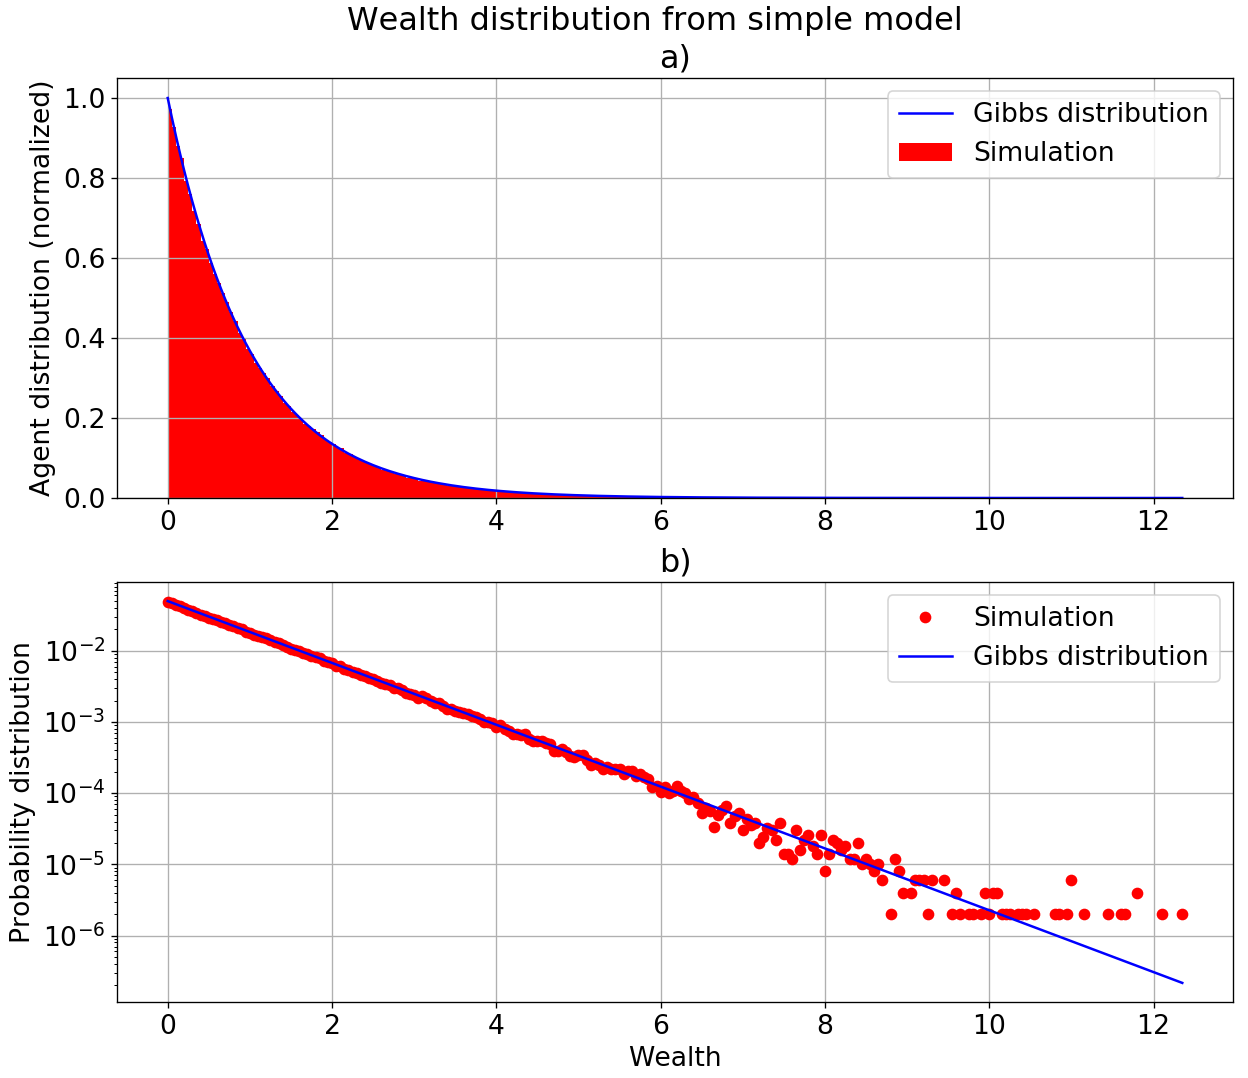
\includegraphics[scale=0.35]{task_b_histogram_agents_500_MCC_1000_N_trans_10000000.png}
\caption{Histogram of equilibrium distribution (a) and corresponding logarithmic plot (b) using the simple model with 500 agents and bin size $\Delta m$ = 0.05. The distribution is clearly linear in (b) as it follows the line of the theoretical Gibbs distribution in blue.   \label{fig:b_hist}}
\end{figure}

\subsection{Equilibrium analysis}
The variance were computed as a function of the number of Monte Carlo cycles to see when the system reached equilibrium. This was done for the simple model with $N_{agents}$ = 500 and $\textrm{$10^7$}$ transactions per cycle. The data can be seen in figure \ref{fig:b_equi}. The variance stabilizes close to a value of $\sigma^2_m$ = 1 after about 1000 Monte Carlo cycles. The number of cycles and transactions per cycle would be increased if access to time and computer power were not limited. 

\begin{figure}[h!]
\centering
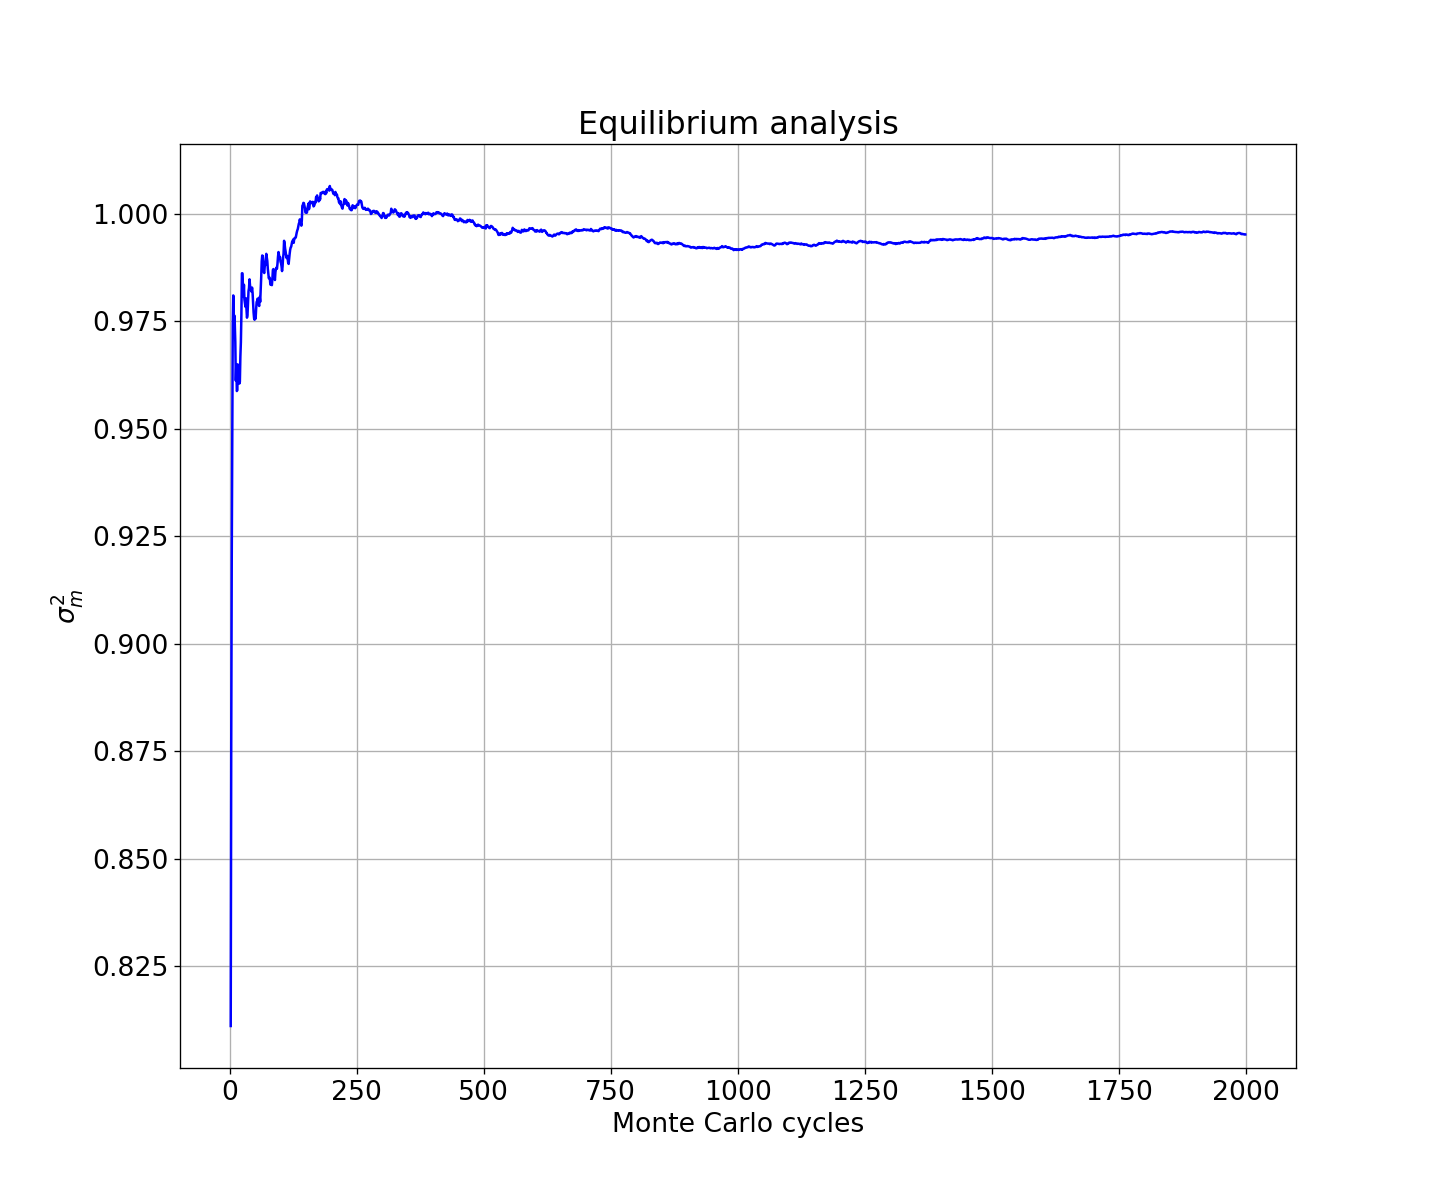
\includegraphics[scale=0.33]{task_b_equi.png}
\caption{Plot of the variance $\sigma^2_m$ as a function of the number of Monte Carlo cycles. The value seemed to stabalize after about 1000 cycles, and this was used as the steady-state situation in all experiments.  \label{fig:b_equi}}
\end{figure}

\subsection{Savings}
The program was now run with the model updated with the savings parameter $\lambda$. It was run for $\lambda$ = [0, 0.25, 0.5, 0.9] with $N_{agents}$ = 500. The results can be seen in the plot in figure \ref{fig:c_prob_dist}. This plot is very close to the plot given in Patriarca et. al \cite{Patriarca}. 

Without savings, the probability distribution decreased with increasing wealth. As the savings rate increased towards $\lambda$ = 0.9, the distribution moved to the right, and eventually peaked at about $m_0$ = 1. Fewer agents ended up with zero wealth, and the maximum wealth for one agent decreased. The peak indicates the expectation value of the wealth and tells us the most probable wealth for an agent. If $\lambda$ was set to 1, the agents would not have any money to trade with, and the plot would show a vertical line at $m$ = 1. 
 
An important point is that the traits from the Gibbs distribution disappears when savings is included, and the graph instead follows the Gamma distribution.

To extract values for the Pareto exponent $\nu$, the top 10th percentile of the graphs in figure \ref{fig:c_prob_dist} was fitted in Python using \textbf{optimize.curve\_fit} from Scipy and the function in equation (\ref{eq:pareto_dist}). The results, including a calculated variance, can be seen in table \ref{tab:savings}.

Low values of $\nu$ will increase the length of the tail and vice verca. Analysing the data, one can see that the Pareto distribution is a good fit when $\lambda \in$ [0, 0.5]. When $\lambda$ = 0.9, the fit is much worse, and it has a very large variance. 


\begin{figure}[h!]
\centering
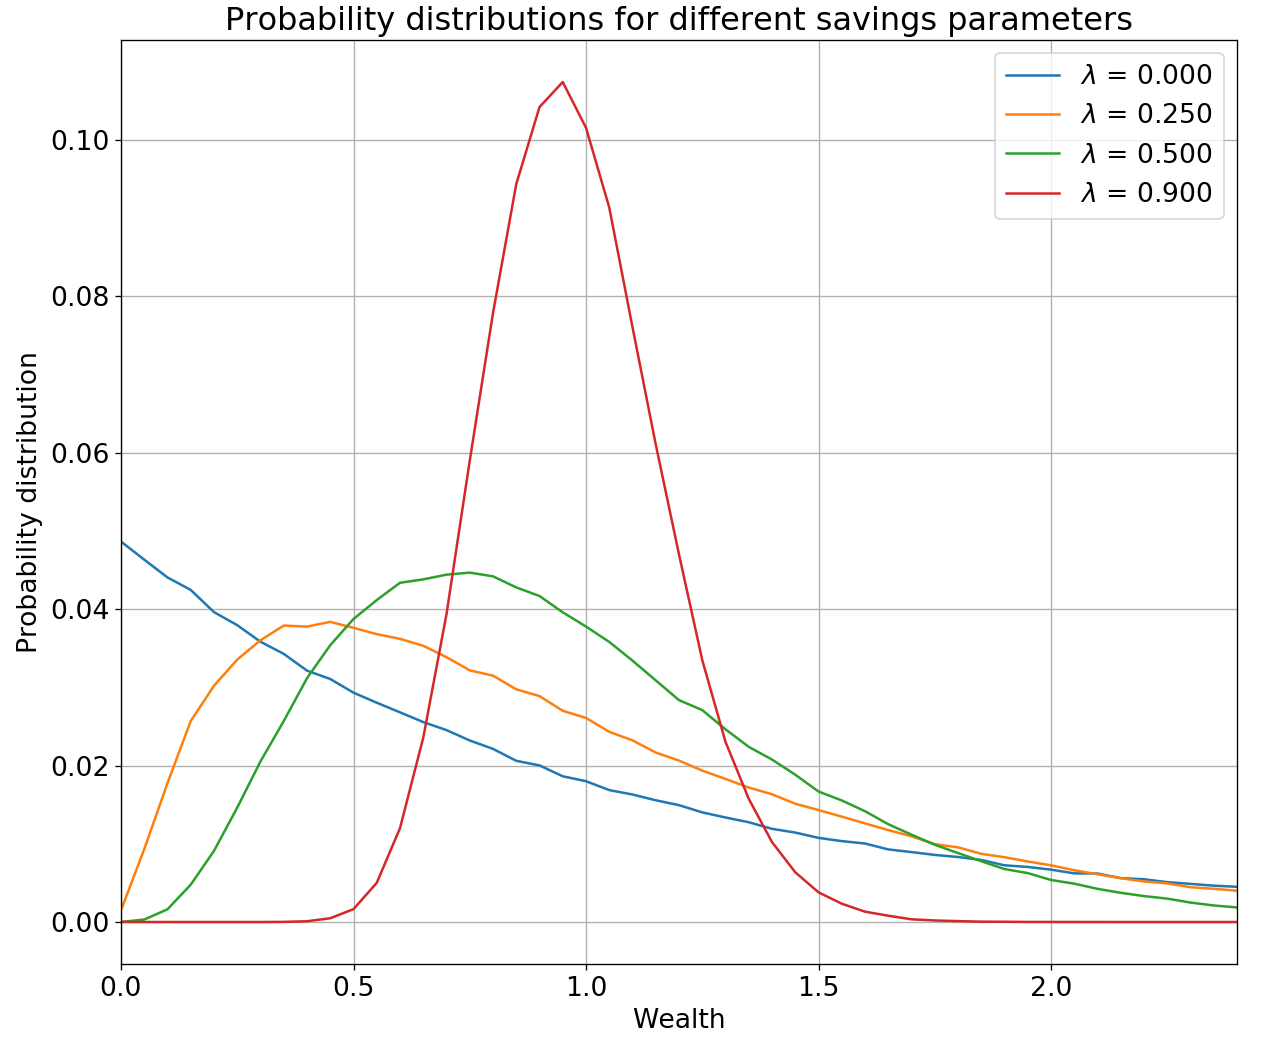
\includegraphics[scale=0.3]{task_c_prob_dist_agents_500_MCC_1000_N_trans_10000000.png}
\caption{ Probability distributions for different values of the savings parameter $\lambda$ with $N_{agents}$ = 500. Without savings, the number of agents decrease with increasing wealth. As the savings rate increase to $\lambda$ = 0.9, the distribution moves to the right and makes a peak at about $m_0$ = 1.  \label{fig:c_prob_dist}}
\end{figure}

\begin{table}[ht!]
\centering
\caption{Estimated Pareto exponents $\nu$ as a function of different values of the savings parameter $\lambda$. The computed variances are also shown. The fit is good up to $\lambda$ = 0.5, but gets much worse when $\lambda$ = 0.9. } \label{tab:savings}
\begin{tabular}{| c | c | c | c | c | c |} \hline
\textbf{$N_{agents}$} & $\lambda$ & $\alpha$ & $\gamma$ &  $\nu$ & $\sigma^2_m$\\ \hline
500 & 0.00 & 0.00 & 0.00 & 4.770 & 0.0074\\ \hline
500 & 0.25 & 0.00 & 0.00 & 6.064 & 0.0068\\ \hline
500 & 0.50 & 0.00 & 0.00 & 7.035 & 0.0033\\ \hline
500 & 0.90 & 0.00 & 0.00 & 44.335 & 1231.5235\\ \hline
\end{tabular}
\end{table}


\subsection{Nearest neighbours}
Including the nearest neighbour parameter $\alpha$ in the program yielded the plots shown in figure \ref{fig:task_d_alpha}. The calculations were done with $N_{agents}$ = [500, 1000] and with $\lambda$ = [0.00, 0.50]. For each of these situations, $\alpha$ was varied from 0.00 to 2.00. The same Pareto fitting as before was also done, and the data is presented in table \ref{tab:nearest}.

An increase in the number of agents from $N_{agents}$ = 500 in figure \ref{fig:task_d_alpha}a and \ref{fig:task_d_alpha}b to $N_{agents}$ = 1000 in \ref{fig:task_d_alpha}c and \ref{fig:task_d_alpha}d increased the total amount of money in the system, making the rich slightly richer. The shape of the distributions was, however, the same for both numbers. 

Increasing the parameter $\alpha$ will decrease the chance of an accepted transaction, and will eventually increase the wealth inequality. Only agents that are financially close will trade, especially for high values of $\alpha$. This means that the poor will trade with the poor, and the rich will trade with the rich. In addition, when an agent becomes very rich, it will most likely stop to trade because he cannot find agents close enough in wealth. 
Most agents will have a wealth $<$ 0, and there will be few rich agents.
This trend is confirmed in figure \ref{fig:task_d_alpha}. A long Pareto-tail can also be seen for some values in the plots corresponding to the low values of $\nu$ when $\alpha \geq$ 1.5 and $\lambda$ = 0.00 in table \ref{tab:nearest}.

In figure \ref{fig:task_d_alpha}b and d, savings are included in the model, and there is now a clear difference from the situation without savings. Firstly, there are much fewer poor agents, and the rich are poorer than before. The most probable wealth is now centered around $m$ = 1. Secondly, the impact of an increased parameter $\alpha$ is reduced, bus it still increases the wealth inequality as before. 

The results are close to the results shown in figure 1 in Goswami and Sen \cite{Goswami}, but one major difference is the kink in the graphs at $m \approx$ 0.01. 



\begin{figure}[h!]
\centering
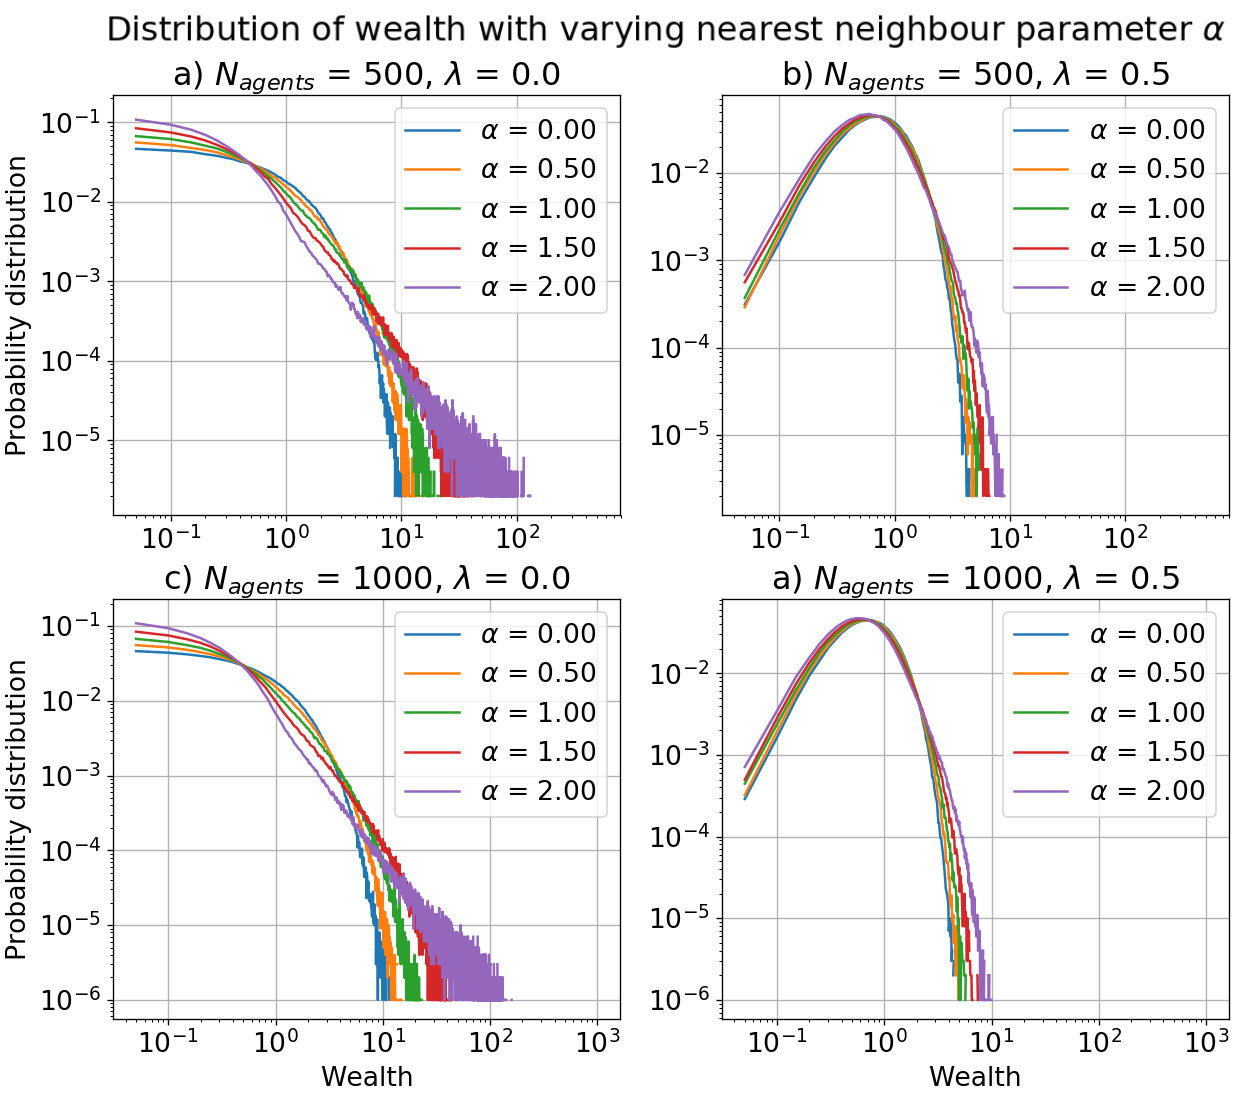
\includegraphics[scale=0.4]{task_d_alpha.png}
\caption{Probability distributions for wealth for different values of $N_{agents}$, $\lambda$ and $\alpha$. In (a) and (b), most agents are poor and a small fraction is very rich. This wealth inequality is reduced when savings are included in (b) and (d). Increasing the parameter $\alpha$ increases wealth inequality in all plots.  \label{fig:task_d_alpha}}
\end{figure}

\begin{table}[h!]
\centering
\caption{Estimated Pareto exponents $\nu$ as a function of different values of $N_{agents}$, $\lambda$ and $\alpha$. The computed variances are also shown. Low values of $\nu$ (long Pareto tail) is found for $\alpha \geq$ 1.5 and $\lambda$ = 0.00.} \label{tab:nearest}
\begin{tabular}{| c | c | c | c | c | c |} \hline
\textbf{$N_{agents}$} & $\lambda$ & $\alpha$ & $\gamma$ &  $\nu$ & $\sigma^2_m$\\ \hline
500 & 0.00 & 0.00 & 0.00 & 4.770 & 0.0074 \\ \hline
500 & 0.50 & 0.00 & 0.00 & 7.035 & 0.0033 \\ \hline
500 & 0.00 & 0.50 & 0.00 & 4.448 & 0.269 \\ \hline
500 & 0.50 & 0.50 & 0.00 & 7.307 & 0.0122 \\ \hline
500 & 0.00 & 1.00 & 0.00 & 3.850 & 0.173 \\ \hline
500 & 0.50 & 1.00 & 0.00 & 6.403 & 0.005 \\ \hline
500 & 0.00 & 1.50 & 0.00 & 2.928 & 0.060  \\ \hline
500 & 0.50 & 1.50 & 0.00 & 5.690 & 0.002 \\ \hline
500 & 0.00 & 2.00 & 0.00 & 2.228 & 0.397 \\ \hline
500 & 0.50 & 2.00 & 0.00 & 5.339 & 0.010 \\ \hline
1000 & 0.00 & 0.00 & 0.00 & 4.709 & 0.004 \\ \hline
1000 & 0.50 & 0.00 & 0.00 & 6.776 & 0.001 \\ \hline
1000 & 0.00 & 0.50 & 0.00 & 4.819 & 0.029 \\ \hline
1000 & 0.50 & 0.50 & 0.00 & 7.039 & 0.004 \\ \hline
1000 & 0.00 & 1.00 & 0.00 & 4.284 & 0.134 \\ \hline
1000 & 0.50 & 1.00 & 0.00 & 6.028 & 0.001 \\ \hline
1000 & 0.00 & 1.50 & 0.00 & 3.245 & 0.066 \\ \hline
1000 & 0.50 & 1.50 & 0.00 & 6.626 & 0.355 \\ \hline
1000 & 0.00 & 2.00 & 0.00 & 2.217 & 0.036 \\ \hline
1000 & 0.50 & 2.00 & 0.00 & 5.486 & 0.013 \\ \hline

\end{tabular}
\end{table}


\subsection{Memory of previous transactions} 
The last effect included in the model is an agent's memory of previous transactions. The power this had on the probability of a transaction was given by the memory parameter $\gamma$. The program was now run with $N_{agents}$ = 1000, $\lambda$ = [0.00, 0.50] and $\alpha$ = [1.00, 2.00]. For each of these situations, the parameter $\gamma$ was varied from 0.00 to 4.00, and the impact this has on wealth distribution can be seen in figure \ref{fig:task_e_gamma}. 

Introducing the memory parameter $\gamma$ without saving and $\alpha$ = 1 (figure \ref{fig:task_e_gamma}a) had a small effect on the distribution. It lowered the probability of being poor and decreased the maximum amount of wealth for the rich. Increasing $\gamma$ further from 1.00 to 4.00 in this situation had almost no effect. 

However, when $\alpha$ = 2 (figure \ref{fig:task_e_gamma}c), the change of $\gamma$ from 1.00 to 4.00 had a slightly stronger impact on the distribution by reducing the wealth of the rich even more. 

Introducing savings (figure \ref{fig:task_e_gamma}b and d) dampened the effects of $\alpha$ and $\gamma$, and also reduced the wealth inequality as before.

The extracted values for the Pareto exponents and the corresponding variances can be seen in table \ref{tab:gamma}. Long pareto tails (low $\nu$) was found when there was no savings, $\alpha$ was high and $\gamma$ was low.

Comparing figure \ref{fig:task_e_gamma} to figure 5 and 6 in Goswami and Sen \cite{Goswami}, one can see that the plots are similar for $\alpha$ = 1.00. For $\alpha = 2.00$ the differences are slightly larger. There is also a kink in the plots at low amount of money which was not seen in this project.

\begin{figure}[ht!]
\centering
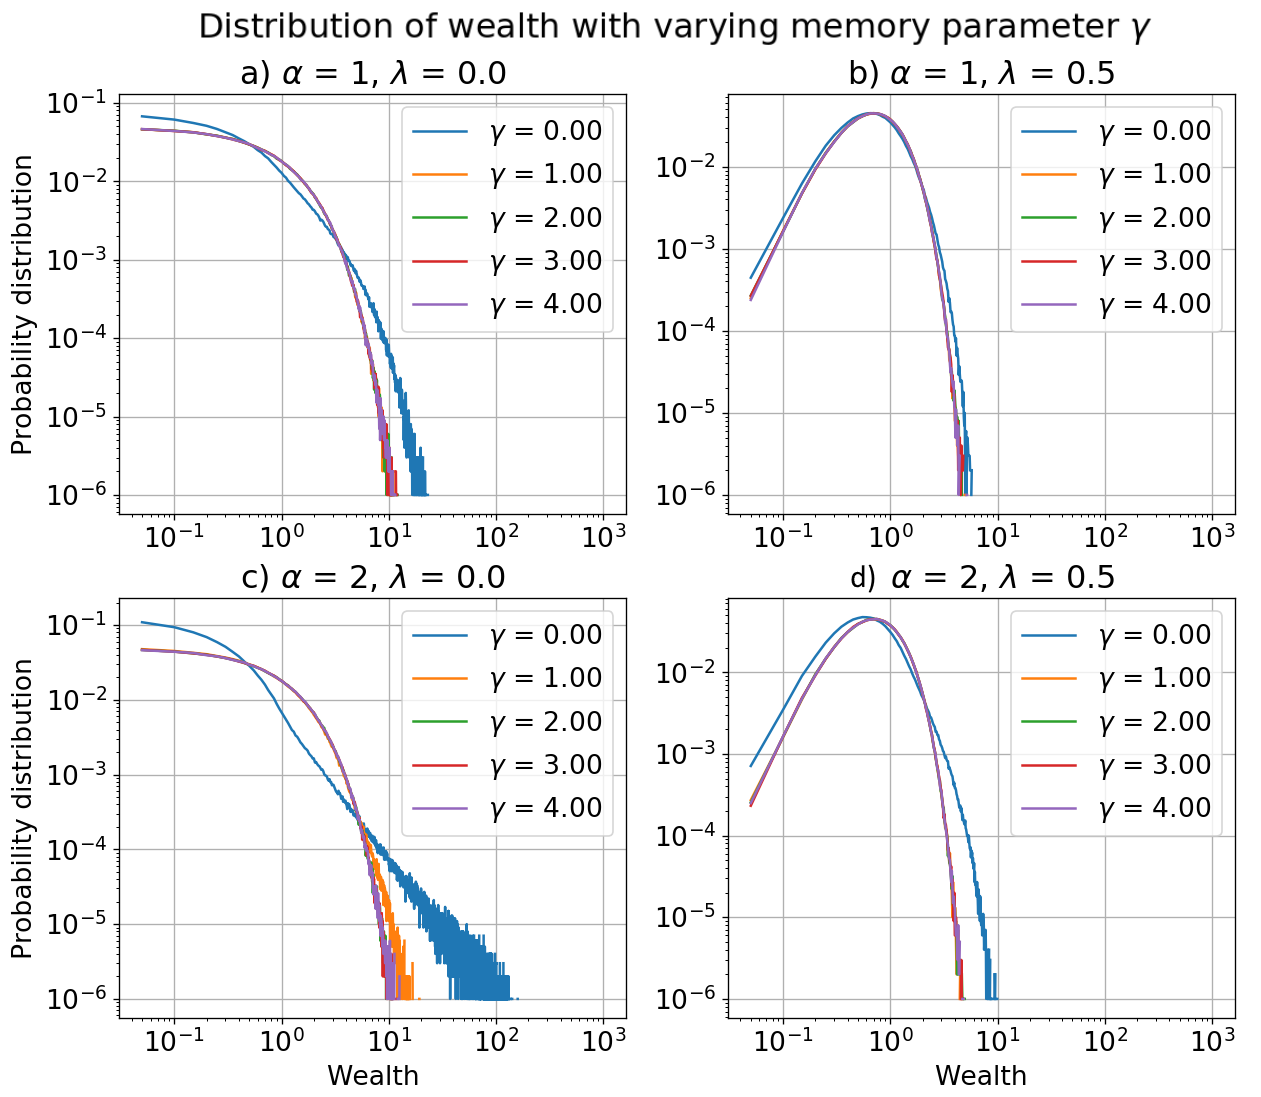
\includegraphics[scale=0.4]{task_e_gamma.png}
\caption{Probability distributions for wealth for different values of $\alpha$, $\lambda$ and $\gamma$. In (a) and (b), most agents are poor, and a small fraction is very rich. This wealth inequality is reduced when savings are included in (b) and (d). Introducing the memory parameter $\gamma$ also leads to a reduction in inequality. Increasing $\gamma$ has a stronger effect when $\alpha$ = 2.    \label{fig:task_e_gamma}}
\end{figure}

\begin{table}[]
\centering
\caption{Estimated Pareto exponents $\nu$ as a function of different values of  $\lambda$, $\alpha$ and $\gamma$. The computed variances are also shown. Long pareto tails (low $\nu$) can be found when there is no savings, $\alpha$ is high and $\gamma$ is low.} \label{tab:gamma}
\begin{tabular}{| c | c | c | c | c | c |} \hline
\textbf{$N_{agents}$} & $\lambda$ & $\alpha$ & $\gamma$ &  $\nu$ & $\sigma^2_m$\\ \hline
1000 & 0.00 & 1.00 & 0.00 & 4.284 & 0.134 \\ \hline
1000 & 0.00 & 1.00 & 1.00 & 4.956 & 0.006 \\ \hline
1000 & 0.00 & 1.00 & 2.00 & 4.994 & 0.012 \\ \hline
1000 & 0.00 & 1.00 & 3.00 & 5.006 & 0.009 \\ \hline
1000 & 0.00 & 1.00 & 4.00 & 5.183 & 0.028 \\ \hline

1000 & 0.00 & 2.00 & 0.00 & 2.217 & 0.036 \\ \hline
1000 & 0.00 & 2.00 & 1.00 & 2.728 & 0.048 \\ \hline
1000 & 0.00 & 2.00 & 2.00 & 3.360 & 0.033 \\ \hline
1000 & 0.00 & 2.00 & 3.00 & 5.166 & 0.017 \\ \hline
1000 & 0.00 & 2.00 & 4.00 & 5.419 & 0.312 \\ \hline

1000 & 0.50 & 1.00 & 0.00 & 6.028 & 0.001 \\ \hline
1000 & 0.50 & 1.00 & 1.00 & 7.190 & 0.001 \\ \hline
1000 & 0.50 & 1.00 & 2.00 & 7.036 & 0.001 \\ \hline
1000 & 0.50 & 1.00 & 3.00 & 6.861 & 0.002 \\ \hline
1000 & 0.50 & 1.00 & 4.00 & 7.240 & 0.004 \\ \hline

1000 & 0.50 & 2.00 & 0.00 & 5.486 & 0.012 \\ \hline
1000 & 0.50 & 2.00 & 1.00 & 7.123 & 0.003 \\ \hline
1000 & 0.50 & 2.00 & 2.00 & 6.922 & 0.002 \\ \hline
1000 & 0.50 & 2.00 & 3.00 & 7.609 & 0.004 \\ \hline
1000 & 0.50 & 2.00 & 4.00 & 6.742 & 0.001 \\ \hline

\end{tabular}
\end{table}





%%%%%%%%%%%%%%%%%%%%%%%%%%%%%%%%%%%%%%
%%%%%%%%%%%Conclusions%%%%%%%%%%%%%%%%%
%%%%%%%%%%%%%%%%%%%%%%%%%%%%%%%%%%%%%%
\section{Conclusion and discussion}
In this project, two articles by Patriarca et. al \cite{Patriarca} and  
Goswami and Sen \cite{Goswami} were used to build a basic model for monetary transactions in an economy where agents could exchange money based on a certain probability. The model was later implemented in C++ using Monte Carlo methods.

The results were close to the results of Patriarca et. al \cite{Patriarca} and Goswami and Sen \cite{Goswami}, but there were some differences. One problem with the articles used in this project is the lack of some experimental data needed to reproduce the given results. It was therefore necessary to do some assumptions.

The basic model without any preferences and memory of the agents yielded an uneven wealth distribution with many poor and a few rich agents. 

When the savings parameter $\lambda$ was introduced, however, it lead to less risk-taking and yielding a narrower distribution of wealth and thus less inequality. This definitely makes the model more realistic, as it would be strange if all agents always traded all their money. It is important to note that the savings model used in this project does not account for time. A more realistic model would have defined what an agent saves over a month or a year. It could thus be useful in to add time dynamics in future developments of this project. 

A high nearest neighbour parameter $\alpha$, on the other hand, caused more people to be poor and rich people to become richer. Thus, wealth inequality increased with an increasing $\alpha$. 

Lastly, the memory parameter $\gamma$ reduced the flow of money, thereby reducing the wealth inequality and dampening the effects of the nearest neighbour interactions. This effect was more clearly seen when the preferential parameter $\alpha$ was high. 

All parameters introduced a Pareto tail to the distribution, and the length of the tail depended on the value of the different parameters. It was found to be long for low values of $\lambda$, high values of $\alpha$ and low values of $\gamma$. A more thorough statistical analysis is needed to fully conclude here.  

If the goal is to reduce wealth inequality in an economy, one should thus aim for trading with small amounts of money (high $\lambda)$, no preference of agents (low $\alpha$) and trading based on previous transaction partners (high $\gamma$).

 


 \clearpage

%%%%%%%%%%%%%%%%%%%%%%%%%%%%%%%%%%%%%%
%%%%%%%%%%%References%%%%%%%%%%%%%%%%%
%%%%%%%%%%%%%%%%%%%%%%%%%%%%%%%%%%%%%%


\begin{flushleft}
\begin{thebibliography}{}

\singlespacing
\small

\bibitem{Patriarca}
  Patriarca, M., Chakraborti, A., \& Kaski, K. (2004). Gibbs versus non-
  Gibbs distributions in money dynamics. \textit{Physica A: Statistical
  Mechanics and its Applications}, 340 (1), pp. 334-339.
 
\bibitem{Goswami}
  Goswami, S., \& Sen, P. (2014). 
  Agent based models for wealth distribution with preference in interaction. 
  \textit{Physica A: Statistical Mechanics and its applications}, 415, pp. 514-524
  
\bibitem{Pareto}
  Pareto, V. (1897), \textit{Cours d'Economique politique}, Lausanne
  

  

  
\end{thebibliography}
\end{flushleft}



\end{document}




















